\subsection{iOS}
	Eine Applikation unter iOS kommuniziert wie unter Android ebenso (Kapitel:
	\ref{sec:app-android}) nicht direkt mit der Hardware sondern mit zwischen der
	App und der Hardware liegenden, nativ gegebenen Schnittstellen, welche wie ein
	Schichtensystem angesehen werden können. Dabei nimmt die Komplexität, ebenso wie
	Nutzungsmöglichkeiten pro hinzu kommender Schicht zu. Durch diese vorgegebene
	Art der Hardwarenutzung wird ein immer gleich bleibender Standard und eine
	gewisse Einheitlichkeit garantiert.
	\begin{figure}[h]
		\centering
		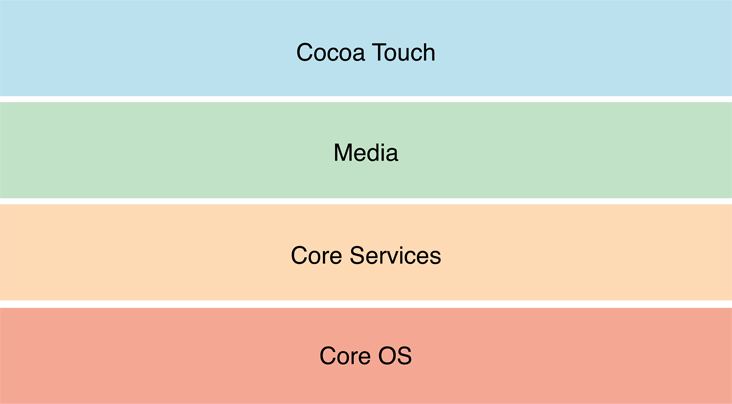
\includegraphics[width=0.5\linewidth]{ios/media/ios-layers.png}
		\caption{Ebenen der iOS Applikationsstruktur}
		\cite{AboutiOSTech2015}
		\label{fig:marcetshare}
	\end{figure}
	
	\subsubsection{Entwicklung einer App}
		Apps für iOS werden in Objective-C (auch: ObjC) und darunter ansässigen
		Sprachen C++ und C verfasst. Zusätzlich ist seit der Vorstellung von
		\textsl{Swift} auf der Apple Entwicklerkonferenz WWDC im Jahre 2014 eine
		neue Hauseigene Sprache dazu gekommen. ObjC ist eine Erweitung von C, welche
		seit dem Erscheinen von Swift immer mehr an Beliebtheit verliert, wohingegen
		Swift seinen Stand bis Juni 2015 im TIOBE-Index deutlich verbessern
		konnte \cite{TIOBE062015}.
		\paragraph{Struktur}
			Applikationen unterliegen der \textsl{model-view-controller} Architektur,
			welche Objekten drei verschiedene Rollen zuweist und den Umgang dieser
			untereinander regelt. Die "`model-Rolle"' ummantelt dabei die Daten und stellt
			Mittel bereit auf diese zuzugreifen und zu verändern. Die "`view-Rolle"' ist
			für Darstellung verantwortlich und reagiert auf Eingaben des Nutzers. Die
			"`controller-Rolle"' ist der Vermittler zwischen view und model und kann
			unter anderem den \textsl{App-Lifecycle} anderer Objekte beeinflussen.
		\paragraph{Entwicklungsumgebung und Lizenzen}
			IOS Apps können nur mit der integrierten Entwicklungsumgebung Xcode
			entwickelt werden. Diese stellt Apple \textsl{OS X Yosemite}
			Benutzern, als auch registrierten Entwicklern kostenlos zur Verfügung.
			Eine Entwickler Lizenz kostet im Jahr 99 US-Dollar. Eine Teilnahme am
			\textsl{iOS Developer Enterprise Program} (Kapitel: \ref{sec:appsigning})
			kostet Firmen jährlich 299 US-Dollar \cite{AppleDev2015}.
		\paragraph{Technologien zur App-Entwicklung}
			Unter IOS werden ein Fülle an Bibliotheken mitgeliefert, welche von der
			tiefen und hardwarenahen Programmierung abstrahieren. Dies ermöglicht mit weniger
			Programmierarbeit Mehr zu erreichen und eventuell komplexe Aufgaben, wie
			Speicherallokation oder Multithreading an tiefere Schichten abzugeben
			\cite{AboutiOSTech2015}.
			Apple empfiehlt eine Arbeitsweise auf möglichst abstrahierter Ebene.
			Nachfolgend wird auf einzelne Bestandteile dieser Schichtenarchitektur
			eingegangen. Es gilt hier anzumerken, dass nur wenige genannt werden, da die
			Nennung und Erläuterung aller den Rahmen dieser Arbeit überlaufen würde.
			\subparagraph{Cocoa Touch Layer}
				Das \textsl{Cocoa Touch Framework} enthält Bibliotheken welche unter anderem
				für das Erscheinungsbild einer App verantwortlich sind. Zusätzlich werden
				Möglichkeiten für Multitasking, Push-Benachrichtigungen, Gestenerkennung und
				viele weitere Schnittstellen auf höherer Programmierebene, wie beispielsweise
				das Twitter-Framework geboten.
			\subparagraph{Media Layer}
				In der \textsl{Medien Ebene} werden Bibliotheken, für
				Audio-, Video- und Bildbearbeitung gespeichert. Außerdem existiert hier die
				Schnittstelle für Apple's \textsl{AirPlay} - einem Video und Audiostreaming
				Dienst für Apple TV und Drittanbieter Lautsprecher beziehungsweise Empfänger.
			\subparagraph{Core Services Layer}
				Auf der dritten Schicht - den Kerndienstleistungen des Systems werden
				Schnittstellen für Peer-to-Peer und andere Netzwerktechnologien angeboten.
				Weiterhin ist es möglicht auf den iCloud Dienst, dem unter Kapitel
				\ref{sec:filesecurity} dokumentierten sicherheitsessentiellen \textsl{Data
				Protection}, sowie die SQLite Unterstützung zurückzugreifen.
			\subparagraph{Core OS Layer}
				Die unterste der vier Schichten liegt am hardwarenahesten und hält somit
				Möglichkeiten auf den Zugriff dieser vor. Dazu zählen das \textsl{Accelerate
				Framework} - unter anderem für Bildbearbeitung und lineare Algebra sowie das
				\textsl{Core Bluetooth Framework} - speziell für die Kommunikation mit
				Bluetooth LE\footnote{LE: Low-Energy} Geräten. Außerdem wird ab iOS 7
				die Unterstützung für native 64-Bit Apps angeboten. Als ein der wichtigsten
				Komponenten soll zuletzt das \textsl{Security Framework} erwähnt werden.
				Dieses bietet Schnittstellen für das Management von Zertifikaten, Richtlinien
				und privaten, sowie öffentlichen Schlüsseln. Außerdem wird das Erstellen von
				Zufallszahlen durch den in Kapitel \ref{sec:crypto-engine}
				vorgestellten \textsl{Random Number Generator} unterstützt, sowie die
				Verwendung von symmetrischer Verschlüsselung durch die unter Kapitel
				\ref{sec:3cc} vorgestellte Bibliothek \textsl{Common Crypto Library}.
